\chapter{AODV}
\label{chap:aodv}

\section{Ejercicio 1.1}

\subsection{¿Qué nodos reenvían el primer paquete RREQ enviado por static1? ¿Y el segundo RREQ? ¿Por qué?}

El primer paquete RREQ enviado por static1 es recibido y reenviado únicamente por los nodos mobile[10] y mobile [12], a pesar de enviarse con intención de alcanzar todos los nodos de la red (Figura \ref{fig:primer_rreq_reception}).
Aunque no es el objetivo de este ejercicio, cabe decir que este comportamiento se debe a la potencia con la que llega a cada nodo la señal y, por supuesto, la posición de cada uno en el plano. Si la señal no llega con potencia suficiente, se considera que el nodo está demasiado lejos para realizar una comunicación efectiva y ya no se intenta decodificar el paquete. La potencia con las que llegan a los nodos las señales también pueden verse en los logs (Figura )
Por otro lado, el paquete solo es reenviado por estos dos nodos y, de igual forma, el segundo RREQ es reenviado por 10, 12, 3, 1, 7, 2

\begin{figure}[H]
    \centering
    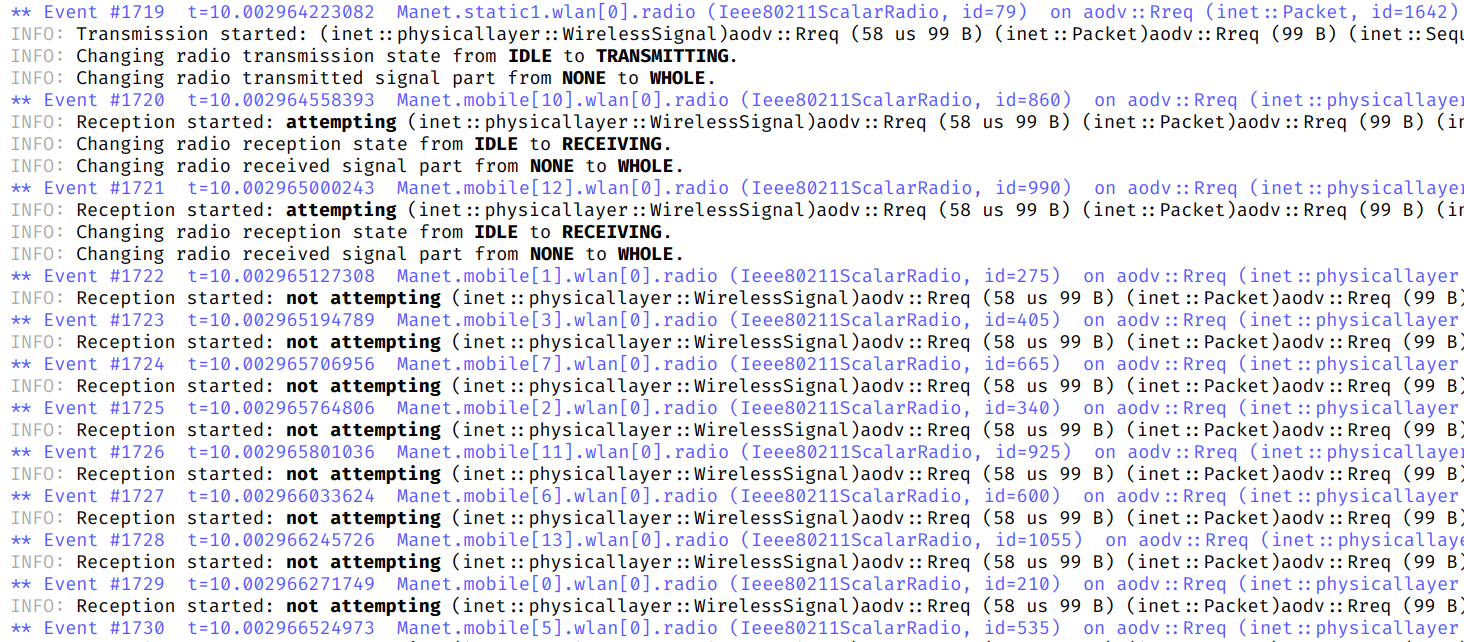
\includegraphics[width=135mm, scale=0.75]{imaxes/ejercicio1_1.png}
    \caption{Logs que muestran el envío del primer RREQ y los nodos que lo reciben}
    \label{fig:primer_rreq_reception}
\end{figure}

\begin{figure}[H]
    \centering
    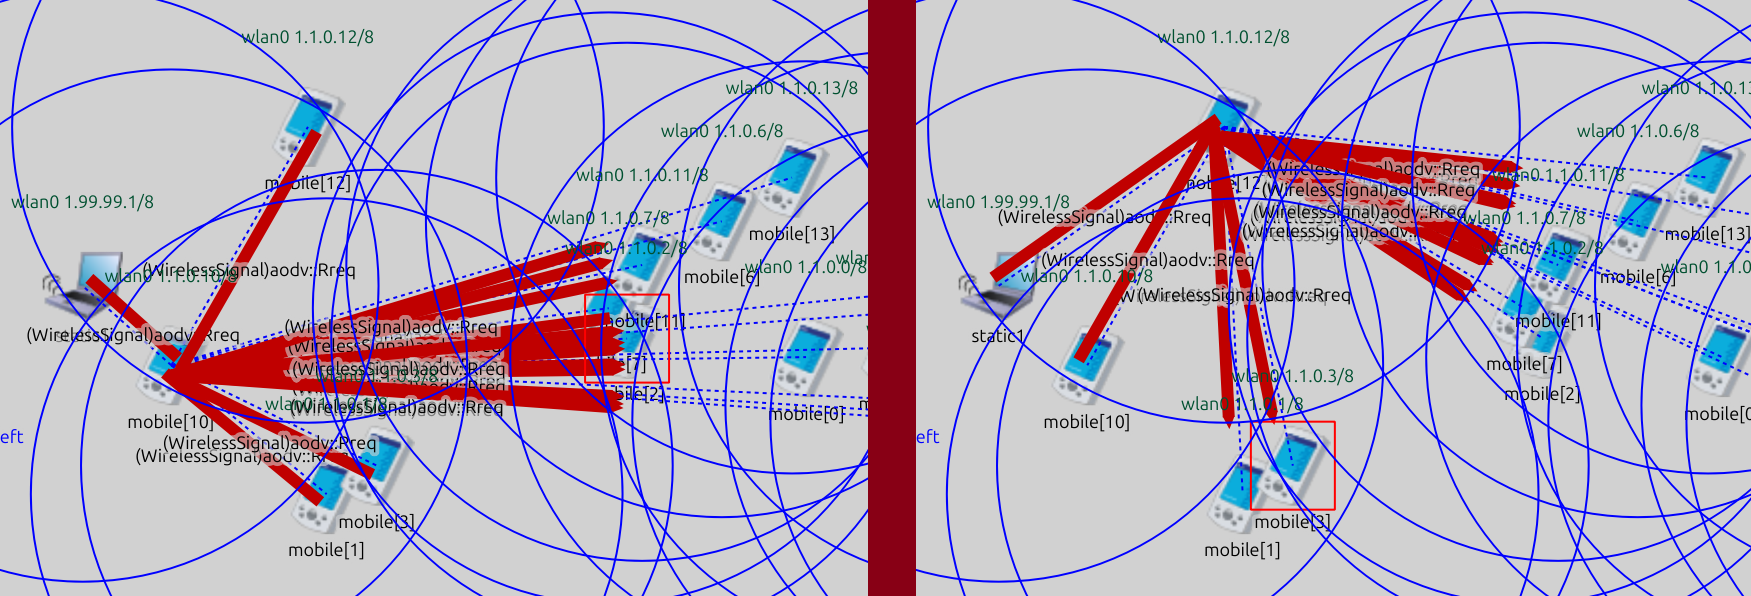
\includegraphics[width=135mm, scale=0.75]{imaxes/ejercicio1_2.png}
    \caption{Nodos que reenvían el primer RREQ (A la izquierda, mobile[10]; A la derecha, mobile[12])}
    \label{fig:primer_rreq_transmission}
\end{figure}

\section{Ejercicio 1.2}

\subsection{Elige el nodo intermedio de la ruta que sigue el primer paquete RREQ que llega a static2. Muestra su tabla
de enrutamiento (vector <Ipv4route *> dentro del módulo ipv4.routingTable) justo antes y justo después de
recibir el primer RREQ. Explica las diferencias y cómo se crean las entradas que aparecen (incluyendo los campos
más importantes).}

\section{Ejercicio 1.3}

\subsection{Haz lo mismo justo antes y justo después del primer RREP.}

\section{Ejercicio 1.4}

\subsection{Tras aplicar la nueva configuración, ¿Cuál es el primer nodo en darse cuenta de la caída? ¿Cómo? Muestra una captura del log del nodo que se da
cuenta que muestre el motivo. ¿Notifica este nodo la caída del nodo?}

\section{Ejercicio 1.5}

\subsection{Muestra el contenido del paquete RERR en Wireshark explicando los campos más importantes. ¿Qué IP
tiene como destino? ¿Por qué?}

\section{Ejercicio 1.6}

\subsection{Explica cómo se propaga el RERR por la red. ¿Qué nodos lo reenvían? ¿Cómo sabe un nodo si debe reenviar
el RERR?}

\section{Ejercicio 1.7} 

\subsection{Muestra capturas de la tabla de enrutamiento de un nodo antes y después de recibir un RERR y explica en
qué cambia.}

\section{Ejercicio 1.8}

\subsection{¿Qué hace static1 al recibir el RERR? Muestra el contenido del siguiente RREQ en Wireshark. ¿En qué cambia
con respecto al de la pregunta 1?}